\subsection{A Fully Statistical Approach to Natural Language Interfaces \cite{Miller1996}}

This paper presents a natural language interface system which is based entirely on trained statistical models. The system consists of three stages of processing: \emph{parsing}, \emph{semantic interpretation}, and \emph{discourse}. Each of these stages is modeled as a statistical process. The models are fully integrated, resulting in an end-to-end system that maps input utterances into meaningful representation frames.

The focus of this paper is to extract sufficient information from each utterance to give an appropriate response to a user's request. The model structure of this paper is described as follows: Given a string of input words $W$ and a discourse history $H$, the task of statistical language understanding system is to search among the many possible discourse-dependent meanings $M_D$ for the most likely meaning $M_0$:
$$M_0 = \mathop{\arg \max}_{M_D} P(M_D | W, H).$$
Let $T$ denote a semantic parse tree, and $M_S$ denote pre-discourse sentence meaning (the sentence meaning without considering the discourse history) we can introduce intermediate levels into the statistical framework:
$$M_0 = \mathop{\arg \max}_{M_D} \sum_{M_S, T} P(M_D | W, H, M_S, T) P(M_S, T | W, H).$$

The representation can be further simplified with the following three assumptions: 1) Neither the parse tree $T$, nor the pre-discourse meaning $M_S$, depends on the discourse history $H$. 2) The post-discourse meaning $M_D$ does not depend on the words $w$ or the parse structure $T$, once the pre-discourse meaning $M_S$ is determined. 3) The probability of words $W$ does not depend on meaning $M_S$, given that parse $T$ is known. Finally, these assumptions yield the following objective function:
$$M_0 = \mathop{\arg \max}_{M_D} (\max_{M_S, T}(P( M_D | H, M_S) P(M_S, T) P(W | T))).$$
\begin{figure}[h]
  \centering
  % Requires \usepackage{graphicx}
  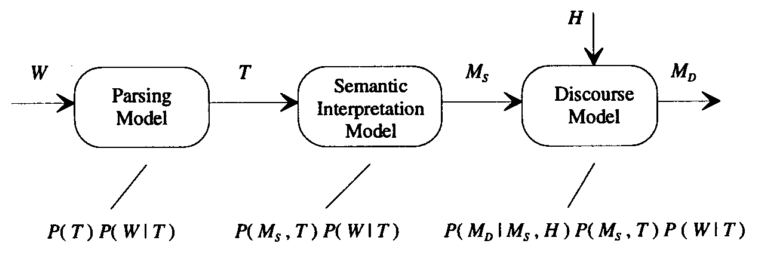
\includegraphics[width=.9\linewidth]{stat_NLI1.png}\\
  \caption{Overview of statistical processing}\label{fig:stat_NLI1}
\end{figure}

This expression corresponds to the computation actually performed by the system which is shown in Figure \ref{fig:stat_NLI1}. The processing proceeds in three stages:
\begin{enumerate}
\item Word string $W$ arrives at the parsing model. The fill space of possible parses $T$ is searched for $n$-best candidates according to the measure $P(T)P(W|T)$. These parses, together with their probability scores, are passed to the semantic interpretation model. The probability $P(T)$ is modeled by state transition probabilities in a recursive transition network, and $P(W|T)$ is modeled by word transition probabilities. Here state transition probabilities have the form $P(state_n | state_{n-1}, state_{up})$, and word transition probabilities have the form $P(word_n | word_{n-1}, tag)$.
\item The constrained space of candidate parses $T$, combined with the full space of possible pre-discourse meanings $M_S$, is searched for $n$-best candidates according to the measure $P(M_s, T)P(W|T)$. These pre-discourse meanings, together with their associated probability scores, are passed to the discourse model. Both pre-discourse and post-discourse meanings in the current system are represented using a simple frame representation (cf. Figure \ref{fig:stat_NLI2}). The problem in this stage is to compute the prior probability of meaning $M_S$ and parse $T$ occurring together. The method of this paper is to embed the instructions for constructing $M_S$ directly into parse $T$. So the probability $P(M_S, T)$ is then simply the prior probability of producing the augmented tree structure.
    \begin{figure}[h]
      \centering
      % Requires \usepackage{graphicx}
      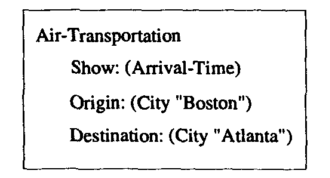
\includegraphics[width=.4\linewidth]{stat_NLI2.png}\\
      \caption{A sample semantic frame}\label{fig:stat_NLI2}
    \end{figure}
\item The constrained space of candidate pre-discourse meanings $M_S$, combined with the full space of possible post-discourse meanings $M_D$, is searched for the single candidate that maximizes $P(M_D | H, M_S)P(M_S, T)P(W|T)$, conditioned on the current history $H$. The discourse history is then updated and the post-discourse meaning is returned. The discourse history $H$ simply consists of the list of all post-discourse frame representations for all previous utterances in the current session. Let $M_P$ denote the last frame in the list. The statistical discourse model maps a 23 element input vector onto a 23 element output vectors. Here $X$ represents the combination of $M_P$ and $M_S$, while $Y$ represents the post-discourse meaning $M_D$. Finally, the probability $P(Y | X)$ is determined by a statistical decision tree model.
\end{enumerate}

In the experimental study, the paper trained and evaluated the system on a common corpus of utterances collected from naive users in the \emph{ATIS} domain. The combined system produced an error rate of 21.6\%, and work on the system was still ongoing. 